\chapter{Gestión de la bibliografía}
La bibliografía se configura en 3 archivos:
\begin{enumerate}
	\item \textit{.../configuracion/05-gestion-bibliografia.tex}: configura la bibliografía y carga las referencias a través de los archivos .BIB.
	\item \textit{.../bibliografia/bibliografia.tex}: carga los comandos de impresión de la bibliografía.
	\item \textit{Archivos .BIB}: son archivos de texto en los que se almacenan las referencias bibliográficas; para la plantilla se guardan en \textit{.../bibliografia/}.
\end{enumerate}
%

La plantilla separa la bibliografía finalmente impresa en 3 partes:
\begin{enumerate}
	\item \textbf{Referencias}: para las obras citadas en el \LaTeX; automatizado.
	\item \textbf{Bibliografía}: para las obras no citadas en el \LaTeX; automatizado.
	\item \textbf{Normativa}: requiere incluir la \textit{keyword} <<nor>> en cada elemento del .BIB que se quiera incluir en esta categoría.
\end{enumerate}
%
\begin{figure}[h]
	\centering
	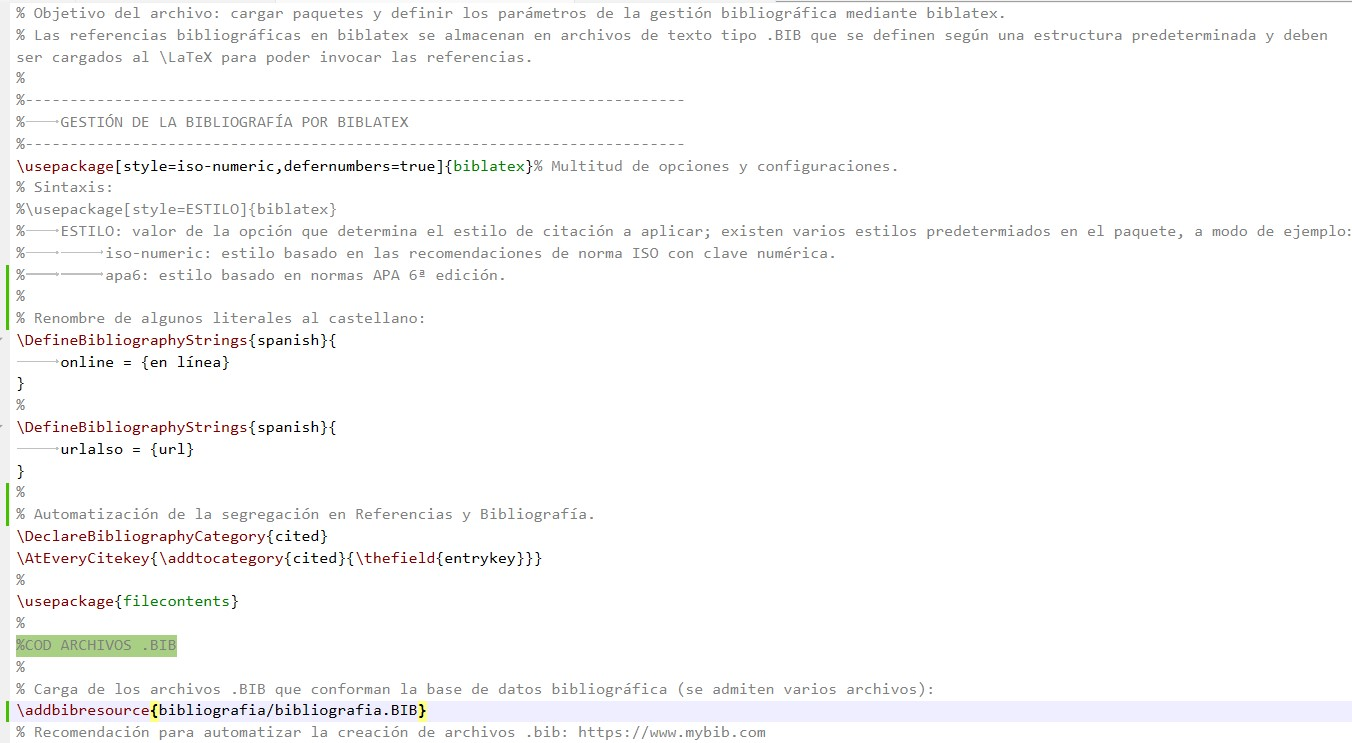
\includegraphics[width=1\linewidth, frame]{cuerpo/cap-referencias/imagenes/05-gestion}
	\caption[Configuración de la gestión bibliográfica.]{Configuración de la gestión bibliográfica. Aquí se carga el paquete y las opciones fundamentales para gestionar la bibliografía, y también los archivos .BIB. Archivo: \textit{.../configuracion/05-gestion-bibliografica.tex}.}
	\label{fig:05-gestion}
\end{figure}
%
\begin{figure}[h]
	\centering
	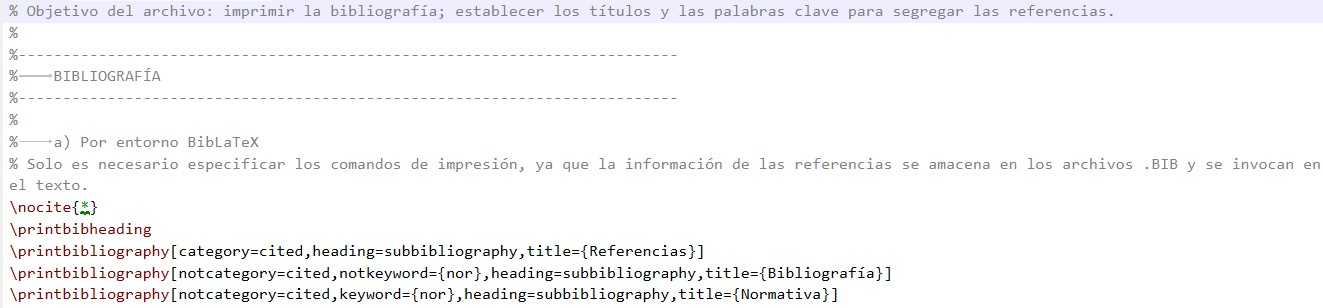
\includegraphics[width=1\linewidth, frame]{cuerpo/cap-referencias/imagenes/biblatex}
	\caption[Configuración de la impresión bibliográfica.]{Configuración de la impresión bibliográfica. Aquí se implementan los comandos de impresión. Archivo: \textit{.../bibliografia/bibliografia.tex}.}
	\label{fig:biblatex}
\end{figure}
%
\begin{figure}[h]
	\centering
	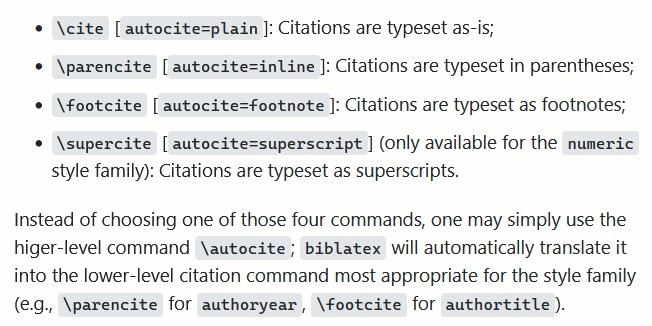
\includegraphics[width=1\linewidth, frame]{cuerpo/cap-referencias/imagenes/modos-cita}
	\caption[Comandos para citar obras.]{Comandos para citar obras.}
	\label{fig:modos-cita}
\end{figure}
%
\chapter{Referencias internas}
Las referencias internas se basan en las etiquetas (\textit{label}). A cada elemento latex (imagen, tabla, sección, párrafo, etc.) se le puede asignar una etiqueta simplemente escribiendo el comando \textit{\textbackslash label\{\}} a su comienzo, o dentro de su entorno. Después, se puede hacer una referencia haciendo una llamada a la etiqueta con el comando \textit{\textbackslash ref\{\}}.

\chapter{Ejemplos de referencias y citas}\label{cap:ejemplos de referencias y citas}
Este es un párrafo sobre Julio César, y en este punto citamos un dato sobre la guerra de las Galias que hemos sacado de una edición de \textit{De bello Gallico}, el dato es X \cite{juliocesar}. Esta guerra acabó tras el asedio de Alesia, con la rendición de los galos liderados por Vercingetorix, escena recreada en el cuadro \ref{fig:rendicion-alesia}. El código empleado se muestra en el fragmento \ref{cod-cesar}.

\begin{figure}[h]
	\centering
	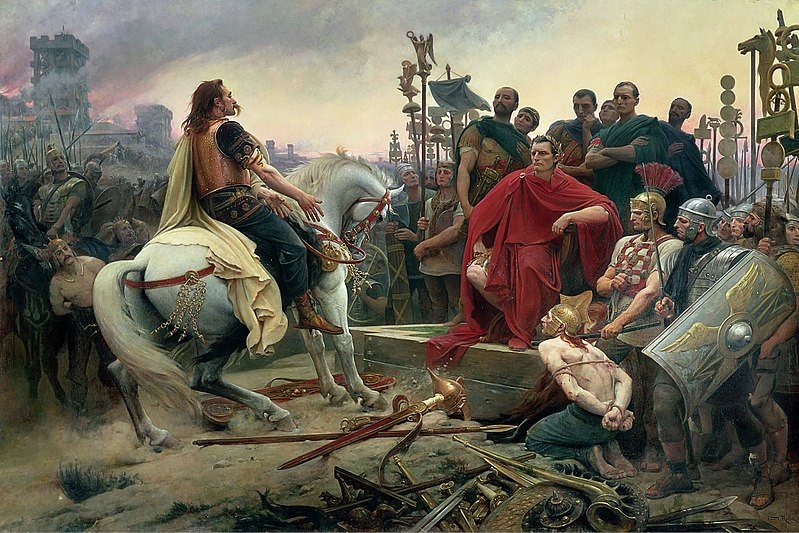
\includegraphics[width=1\linewidth, frame]{cuerpo/cap-referencias/imagenes/rendicion-alesia}
	\caption[Vercingetorix rinde sus armas a los pies de Julio César.]{Vercingetorix rinde sus armas a los pies de Julio César. Cuadro de Lionel Royer. Fuente: \cite{cuadro-rendicion-alesia}.}
	\label{fig:rendicion-alesia}
\end{figure}
%
\newpage
\lstinputlisting[frame={single}, language={[AlLaTeX]TeX},, label={cod-cesar}, caption=Código empleado en el capítulo \ref{cap:ejemplos de referencias y citas}.]{cuerpo/cap-referencias/codigos/cesar.txt}